
\chapter{Introduction} 
\label{chap:Introduction}

\section{Motivation}
\label{sec:Intro_Motivation}
Recently, NAND flash memory is widely used as a storage device from
embedded systems to high-end enterprise servers. Because of its many attractive
characteristics for mobile storage devices such as light weight, low
power consumption, durability, and high performance, it has been widely
used for mobile embedded systems. In addition to the advantages, as the
cost per byte is falling while the storage capacity is increased, large-capacity
NAND flash memory devices such as solid state drives (SSDs) are more
commonly employed for high-end desktops and enterprise storage servers.

\begin{figure*}[b]
	\centering
	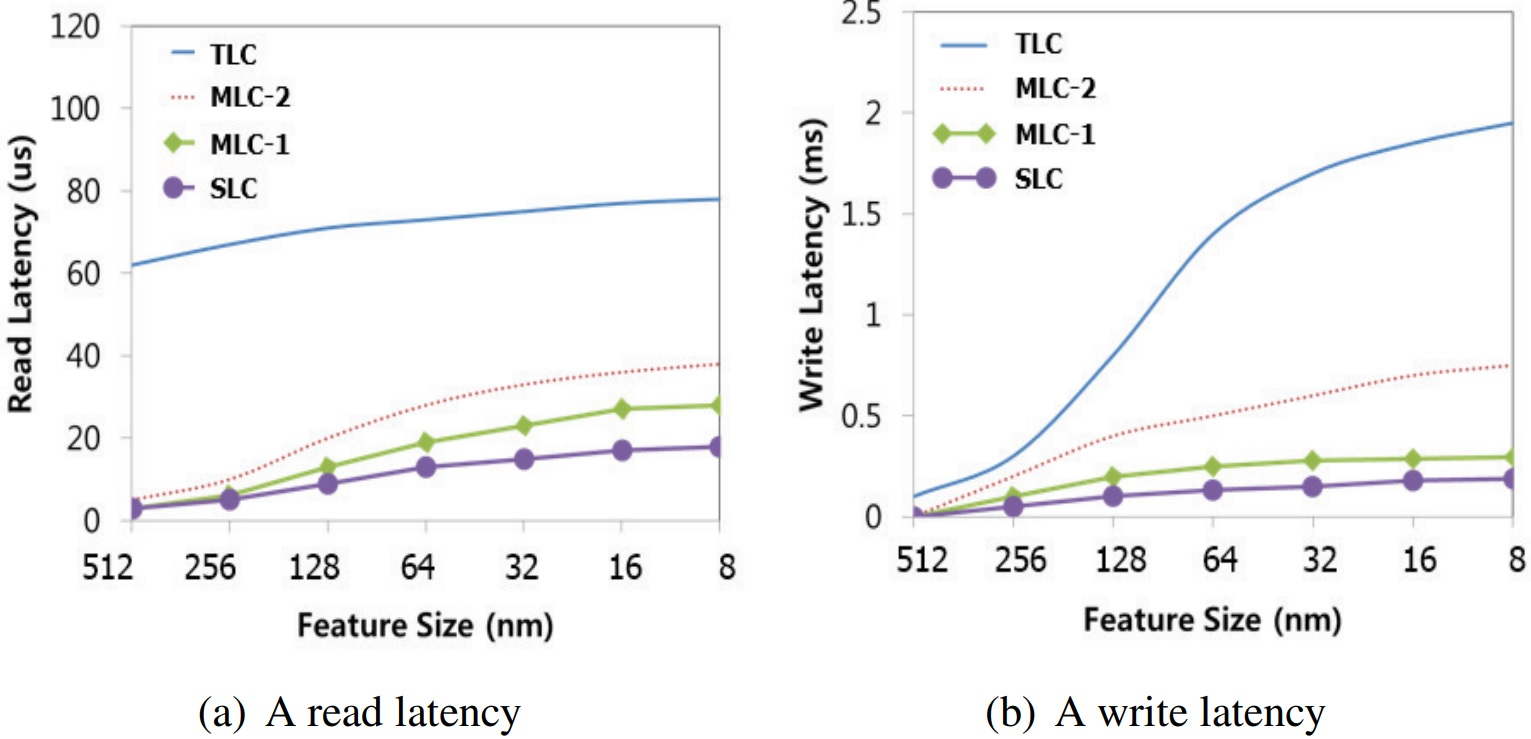
\includegraphics[width=0.8\textwidth]{figure/intro/latency_trend}
	\caption{Trends of read and write speeds under various NAND flash chips.}
	\label{fig:latency_trend}
\end{figure*}


However, as NAND flash memory technology scales down to 10-nm
and below, performance of NAND flash memory is also getting worse.
Figure~\ref{fig:latency_trend} shows a tendency of read and write speeds of NAND block under
various feature sizes. In Figures~\ref{fig:latency_trend}(a) and (b), 
the x-axis denotes a feature
size of NAND chip, and the y-axis represents the latencies of read and
write operations, respectively. As shown in Figures~\ref{fig:latency_trend}(a) and (b), 
both read and write operations are slower as the density of NAND flash memory is
increased. In the future, as NAND flash memory is scaled down and the
number of bits per cell is increased, the data reliability and performance
degradation problems will be even more critical to NAND-based storage
systems.

Moreover, the limited endurance of NAND flash memory, which have declined
further as a side effect of the recent advanced device technologies,
is emerging as major barrier to the wide adoption of SSDs. For example,
although the NAND capacity per die doubles every two years, the actual 
lifetime of SSDs does not increase as much as projected because the
maximum number of program/erase cycles has declined~\cite{MooresLaw}.
In order for SSDs to be widely adopted, the issues concerning NAND endurance 
should be properly resolved.

\subsection{Garbage Collection Problem}
Because of the performance degradation of high-density NAND flash
memory, the overhead of garbage collection (GC) is increased. In NAND
flash-based storage systems, garbage collection is required when there are
not enough free blocks to write new data because NAND flash memory does
not allow an in-place update operation. If data are updated in NAND flash
memory, an FTL stores the newly requested data in another page. Since
the previously written data remain as invalidated data in the NAND flash
memory, a garbage collection process is triggered by the FTL in order to reclaim
the blocks with the invalidated data so that new data can be stored into
NAND flash memory. A garbage collection procedure involves several read,
write, and erase operations. Since each operation of NAND flash memory is
atomic, the FTL cannot process the next request from a file system while an
operation is processed during a garbage collection process. 
Because of the performance degradation of read and write
operations in high-density NAND flash memory, the response time of each
I/O request can be elevated when the request is conflicted with a garbage
collection process, thus decreasing file system performance. In other words,
the whole system is likely to be delayed for a longer time compared to lowdensity
NAND flash memory due to the slow extra copies and erases during
garbage collection processes. Since such problem can be aggravated in the
future high-density NAND flash memory, an efficient garbage collection algorithm
is becoming more and more important.

In order to minimize the garbage collection overhead, many techniques
have been proposed~\cite{FTL}. Regardless of garbage collection algorithms used,
moving valid data from selected victim blocks to new blocks during garbage
collection takes a significant portion in the total execution time of a garbage
collection algorithm. Therefore, reducing the total number of copied data
from the victim blocks is a key factor in improving the performance of a
garbage collection algorithm. To reduce the amount of copied data from the
victim blocks, a common approach is to separate data based on their characteristics
so that the number of dead blocks (which have no valid data) or
near-dead blocks (which have few valid data) can be increased. The more
dead or near-dead blocks are generated, the more likely that they can be selected
as victim blocks during garbage collection, thus reducing the garbage
collection overhead.

One of the most widely used data separation heuristics is to classify
data based on their update frequency. This data separation technique classifies
data based on their write temporal locality, and it treats data with different
temporal locality in a different way~\cite{HotCold}. The assumption of this
technique is that data with high write temporal locality are likely to be updated
soon by successive update requests, and hence the number of dead
blocks increases if data with high locality are clustered in the same block.
The simplest version of this locality-based data separator divides data into
two groups, hot data and cold data according to the number of updates in a
given time period. By storing hot data in hot blocks, they are more likely to
be dead blocks.

\subsection{Limited Endurance Problem}

The limited endurance of NAND flash memory, which have
declined further as a side effect of the recent advanced device technologies,
is emerging as another major barrier to the wide adoption of SSDs. (NAND endurance
is the ability of a memory cell to endure program/erase (P/E) cycling, and is
quantified as the maximum number $MAX_{P/E}$ of P/E cycles that the cell can tolerate
while maintaining its reliability requirements.) 
Since the reduction in the $MAX_{P/E}$ seriously limits the overall lifetime of flash-based SSDs,
the issues concerning the lifetime of SSDs should be properly resolved for SSDs to be commonly 
used in enterprise environments.

Since the Lifetime $L_C$ of an SSD with the total capacity $C$ is proportional to 
the maximum number $MAX_{P/E}$ of P/E cycles, and is inversely proportional to the
total written data $W_{day}$ per day, $L_C$ (in days) can be expressed as follows
~\cite{DPES}(assuming a perfect wear leveling):
\[L_C = \frac{MAX_{P/E} \times C}{W_{day} \times WAF}\],
where $WAF$ is a write amplification factor which represents the efficiency of an FTL
algorithm. Since $MAX_{P/E}$ and $C$ is determined when the device is manufactured,
we should reduce the $W_{day}$ and $WAF$ to improve the lifetime of SSDs.
Many existing lifetime-enhancing techniques have been focused on reducing $WAF$
by increasing the efficiency of an FTL algorithm. For example, by avoiding
unnecessary data copies during garbage collection 
using the multi-stream feature, $WAF$ can be reduced.
In order to reduce $W_{day}$, various system-level techniques were proposed.
For example, data deduplication, data compression, and write traffic 
throttling are such techniques.

Most existing studies, however, are based on the the single I/O layer such as 
block I/O, device driver, and SSD firmware so their effectiveness is limited.
In order for NAND flash-based storage devices to be broadly adopted in
various computing environments, therefore,
new approaches that properly address the lifetime problem of recent
high-density NAND flash memory are highly required.

\begin{comment}
%----------------------------------------------------
As the price-per-byte of NAND flash memory is rapidly decreasing,
NAND flash-based solid-state drives (SSDs) are emerging as a viable high-performance storage solution
for laptops, desktop PCs and high-performance enterprise systems.
%The poor write endurance of NAND flash memory, however, is emerging as one of the main obstacles 
%for wider adoption of SSDs in various computing environments.
%In NAND flash memory, reads and writes are performed in a unit of a page.
%Because of its `erase-before-write' nature,
%a block consisting of multiple pages must be erased before programming (or writing) new data to it.
%Unfortunately, as the semiconductor process is scaled down and the multi-level cell (MLC) technology is introduced,
However, as NAND flash memory technology scales down to 20-nm and below, storing data reliably in NAND flash memory
gets a key design challenge of NAND-based storage systems. 
For example, the number of program/erase (P/E) cycles allowed for each block is significantly reduced in recent triple-level cell (TLC)
NAND technology.
While older 5x-nm single-level cell (SLC) NAND flash memory can support about 10 K P/E cycles, recent 2x-nm TLC NAND flash memory
can barely support about 1 K P/E cycles~\cite{tlc}.
%the number of P/E cycles is reduced to 3K~\cite{mlc1}. %~\cite{mlc1,mlc2}.
%As a result, the reduction in the number of P/E cycles seriously limits the overall lifetime of flash-based SSDs.
%----------------------------------------------------
\end{comment}

\section{Dissertation Goals}
In this dissertation, we propose system-level approaches that improve 
the lifetime of NAND flash-based storage devices, which overcomes the limitations
of the existing techniques. More specifically, our primary goal is to understand 
high-level information of applications, such as the 
I/O context of dominant I/O activities,
and then develop the lifetime improvement approaches that efficiently exploit such
high-level information at various system levels ranging from a system call layer 
to a flash controller.

First, we propose a system-level approach to reduce WAF that exploits
the I/O context of an application to increase the data lifetime prediction
for the multi-streamed SSDs. 
%By extracting program contexts during runtime, data-to-stream mapping is done automatically.
Thus, it can effectively separate data with
short lifetimes from data with long lifetimes to improve the efficiency of garbage collection.
Moreover, when data mapped to the same
stream show large differences in their lifetimes,
long-lived data of the current stream are moved to 
its substream during garbage collection.

Second, we present a write traffic reduction technique to improve the lifetime of 
SSD by exploiting data similarity of I/O context of an application. 
We analyze the likelihood of duplicate data for each I/O context and 
selectively apply deduplication technique to highly duplicated context.
By avoiding disturbance of unique context,
we can increase the chance of finding duplicate data and 
decrease the write latency.
With the decreased fingerprinting overhead, we propose new deduplication technique
to increase the overall
deduplication ratio\footnote{The percentage of identified duplicate writes}
by introducing sub-page chunk. 
It resolves technical difficulties caused by its finer granularity, i.e., 
increased memory requirement and read response time. 

\section{Contributions}
In this dissertation, we present two system-level techniques to improve the 
lifetime of NAND flash-based storage devices using program context characteristics. 
The contributions of this dissertation can be summarized as follows:

\begin{itemize}
\item 
We showed that data lifetime and duplicate data have different characteristics depending on the I/O activity.
We also implemented program context extraction to effectively use the I/O activity for optimization.

\item 
We propose a fully automatic stream management
technique, PCStream, which can work efficiently for general
I/O workloads with heterogeneous write characteristics. PCStream
is based on the key insight that stream allocation decisions
should be made on dominant I/O activities. By identifying
dominant I/O activities using program contexts, PCStream
fully automates the whole process of stream allocation
within the kernel 

\item
We propose a selective deduplication using program contexts
with a fine-grained deduplication technique for flash-based SSDs, called \textsf{\small FineDedup}.
The proposed FineDedup technique is different from other existing deduplication techniques
in that it increases the likelihood of finding duplicates
by using a finer deduplication unit
which is smaller than a single page (e.g., one fourth of a single page).
Moreover, FineDedup analyzes the likelihood of finding duplicate data for each PCs.
For low dedup ratio PCs, FineDedup skips the deduplication step to avoid unnecessary 
fingerprinting overhead.

\item
We implement the proposed techniques in the Linux kernel and our in-house flash storage
prototype. Then, we evaluate their effects on performance and lifetime using 
various real-world applications on the real SSD device as well as the emulator.
 
\end{itemize}

\section{Dissertation Structure}
This dissertation is composed of five chapters. The first chapter is the introduction
of theh dissertation, while the last chapter serves as conclusions with a summary
and future work. The three intermediate chapters are organized as follows:

Chapter 2 provides the background for multi-streamed SSDs and data deduplication
techniques as well as the overall architecture of NAND flash-based storage devices.
We also describe the existing lifetime improvement techniques for flash-based devices,
focusing on multi-streamed SSDs and deduplication techniques which are highly related
to our proposed techniques.

Chapter 3 presents the definition of program contexts and how to extract them.
Also, distinct lifetime patterns for PCs and duplicate data patterns are shown.

In Chapter 4, we present a new data separation technique, called PCStream, 
for multi-streamed SSDs. We explain the relationship of dominant I/O activities
with data lifetime patterns. By exploiting distinct lifetime patterns of I/O activities,
we can achieve high reduction in WAf.

Chapter 5 introduces a fine-grained deduplication technique, called FineDedup, for NAND
flash-based storage devices. We describe the patterns of duplicate data with in a page.
Finally, we show how effective the proposed technique is in terms of write traffic reduction.

